\subsection{Abstract Equation}
\paragraph{Stochastic Differential Equations}
Assume we are given a drift $\mu:[0,1]\times \mathbb R^d\to\mathbb R^d$ and diffusivity $\sigma:[0,1] \times \sR^d \to \mathbb R^{d\times d}$, we consider the SDE
\begin{align}\label{eq:sde_abstract}
  \mathrm dX_t
  &=
    \mu(t, X_t)\mathrm d t
    +
    \sigma(t, X_t) \mathrm d W_t,
    \quad
    X_0 \sim p_0,
\end{align}
where $W_t$ is a standard Brownian motion and $X_0$ is distributed according to $p_0$.

\paragraph{The Fokker-Planck Equation}
To solve the SDE \eqref{eq:sde_abstract}, i.e., to obtain the dynamics of the associated probability density we can solve the \emph{Fokker-Planck equation}, which is given by
\begin{align}\label{eq:fokker_planck_abstract}
  \partial_t p
  +
  \operatorname{div}(p\mu)
  -
  \frac12 \operatorname{tr}(\sigma \sigma^\top\nabla^2 p)
  =
  0,
  \quad
  p(0) = p_0.
\end{align}
Note that for every time-point $p(t,\cdot)$ is a probability density on $\mathbb R^d$, hence $p:[0,1]\times\mathbb R^d \to \mathbb R$. The PINN loss of the Fokker-Planck equation is, after parametrizing $p$ as a neural network $p_{\vtheta}$, given by
\begin{align*}
  L^{\textrm{FP}}(\vtheta)
  &=
    \frac{1}{2N}
    \sum_{n=1}^{N}
    \big[
    \partial_t p_{\vtheta}
    +
    \operatorname{div}(\mu p_{\vtheta})
    -
    \frac12 \operatorname{tr}(\sigma\sigma^\top\nabla^2 p_{\vtheta})
    \big]^2
    (\vx_n)
  \\
  &+
    \frac{1}{2 N_0}
    \sum_{n=1}^{N_0}
    \big[
    p_{\vtheta}(\vx_n^0) - p_0(\vx_n^0)
    \big]^2.
\end{align*}
To make sampling tractable, we replace $\mathbb R^d$ by a compactum\footnote{If this is really the smartest way to handle infinite domains is not clear to me, I think it seems rather naive, but I am not familiar enough with the literature.}, say $[-L, L]^d$ for suitable $L>0$. Then we draw $\vx_n \sim [0, 1] \times [-L, L]^d$ and $\vx_n^0 \sim \{0\} \times [-L, L]^d$. Our experiments use $L=5$.


\paragraph{The Fokker-Planck Equation in Log-Space}
For numerical stability, transferring this PDE into $\log$-space is commonly employed. The ansatz $q = \log p$ lets us solve \eqref{eq:fokker_planck_abstract} via the \emph{nonlinear} PDE (which is a special case of a Hamilton-Jacobi-Bellman equation) given by
\begin{align}\label{eq:log_fokker_planck_abstract}
  \partial_t q
  +
  \operatorname{div}(\mu)
  +
  \nabla q \cdot \mu
  -
  \frac12 \| \sigma^\top \nabla q \|^2
  -
  \frac12 \operatorname{tr}(\sigma \sigma^\top\nabla^2 q)
  =
  0,
  \quad
  q(0) = \log p_0.
\end{align}
Again, parametrizing $q$ by a neural network $q_\vtheta$ yields for the PINN loss of \eqref{eq:log_fokker_planck_abstract}
\begin{align*}
  L^{\textrm{logFP}}(\vtheta)
  &=
    \frac{1}{N}
    \sum_{n=1}^{N}
    \big[
    \partial_t q_{\vtheta}
    +
    \operatorname{div}(\mu)
    +
    \nabla q_\vtheta \cdot \mu
    -
    \frac12 \| \sigma^\top\nabla q_\vtheta \|^2
    -
    \frac12 \operatorname{tr}(\sigma\sigma^\top\nabla^2 q_{\vtheta})
    \big]^2
    (\vx_n)
  \\
  &+
    \frac{1}{N_0}
    \sum_{n=1}^{N_0}
    \big[
    q_{\vtheta}(\vx_n^0) - \log p_0(\vx_n^0)
    \big]^2.
\end{align*}
We draw $\vx_n \sim [0, 1] \times [-L, L]^d$ and $\vx_n^0 \sim \{0\} \times [-L, L]^d$ as before.

\subsection{Concrete Examples}
\paragraph{A Sanity Check Example (\texttt{isotropic\_gaussian})}
Set the drift $\mu$ to $\mu(t,x) = -1/2x$ and choose $\sigma=\sqrt 2 I$. As initial condition we use $p_0 \sim \mathcal N(0,I)$. For this concrete data, the Fokker-Planck equation is
\begin{subequations}
  \begin{align}\label{eq:fokker-planck-isotropic-gaussian}
    \partial_t p(t, x)
    -
    \frac12 \operatorname{div}(xp(t,x))
    -
    \Delta p(t,x)
    =
    0,
    \quad
    p(0) \sim \mathcal N(0, I).
  \end{align}
  The solution to this equation is given by
  \begin{equation}
    p^*(t, x) \sim \mathcal N(0, \exp(-t)I + (1 - \exp(-t)) 2 I).
  \end{equation}
\end{subequations}

The logarithmic Fokker-Planck equation for this data is
\begin{equation}\label{eq:log-fokker-planck-isotropic-gaussian}
  \partial_t q(t,x)
  -
  \frac d2
  -
  \frac12\nabla q(t,x)\cdot x
  -
  \| \nabla q(t,x) \|^2
  -
  \Delta q(t,x)
  =
  0,
  \quad
  q(0) = \log(p^*(0)),
\end{equation}
with solution $q^* = \log(p^*)$.

\begin{itemize}
\item The fact that $\sigma$ is a diagonal matrix simplifies the term with the second partial derivatives. In general, we cannot assume this, so it is interesting to think about Taylor mode differentiation in this context. I know it will work, I am wondering how much we gain over backprop here, especially in high dimensions.

  Let's look at $\Tr(\mA \mA^\top \nabla^2 q) = \sum_i \sum_j \sum_k \emA_{i,j} \emA_{k,j} (\nabla^2_{k,i} q) \coloneqq \sum_i \sum_k \emB_{k,i} (\nabla^2_{k,i} q)$ where $\mB \coloneqq \mA \mA^\top$. This is just a weighted sum of second-order partial derivatives. As we explain at the end of \Cref{sec:taylor-mode-AD}, we can derive forward propagation rule which looks similar to the forward Laplacian (and I believe has the same computational complexity, but I will need to write down the exact expression).


\item A simple trick let's us encode the initial conditions directly into the neural networks ansatz:
  \begin{equation}
    \tilde p_\theta = t p_\theta + \mathcal N(0, I).
  \end{equation}
  This guarantees that our neural network ansatz, now called $\tilde p_\theta$ exactly satisfies the initial condition. This trick typically helps and should always be employed\footnote{We did not do that for the other equations because the Poisson and the heat equation are interesting in potentially complicated domains, where such a trick for the boundary conditions would be very difficult to realize in practice. Thus it should be considered ``cheating''. The situation for the Fokker-Planck is different. Here this trick---if helpful---should always be used.}.
\item The Fokker-Planck equation is a PDE on an unbounded domain, typically $\mathbb R^d$, so we need to artificially restrict ourselves to some compact interval. This causes issues with numerical accuracy and the optimization.
\item The Fokker-Planck equation is interesting for PINNs as it frequently appears for high-dimensional settings. Hence grid-based methods are intractable. This is our motivation to look at this equation.
\item The example above will not work well for high dimensions when using the original Fokker-Planck equation. The log-space ansatz is expected to help and seems to be the standard in the community.
\end{itemize}

\subsection{Literature}
\begin{itemize}
\item \cite{hu2024score} PINNs for Fokker-Planck in dimensions 100 and 250. The paper discusses the original Fokker-Planck equation, the log space version and another reformulation based on the score -- which we haven't looked into yet. Our sanity check example is motivated from Section 4.1.1 in this paper.
\item \cite{wang20222} claimes that the log space Fokker-Planck equation should not be trained with an $L^2$ loss because the $L^2$ loss does not control the error. I am unsure if this is relevant for numerical experiments, though. We can have it in mind if we manage to drive the loss down but don't observe the same for the error.
\end{itemize}

% tuning protocol: Bayesian (copy search spaces from Poisson+Bayes)
% exp35: 1+1 FP, single-layer net
% exp36: 9+1 log-FP, D~100k
% exp37: 99+1 log-FP, D~1M
% exp38: group plot for FPs

\subsection{(1/9/99)+1-d (Logarithmic) Fokker-Planck Equations with Random Search}

Here, we consider three different Fokker-Planck equations and use random search as tuning protocol:
\begin{enumerate}
\item The $1+1$-d Fokker-Planck equation from \Cref{eq:fokker-planck-isotropic-gaussian} whose solution we model with a small $2 \to 64 \to 1$ tanh-activated MLP with $D=\num{257}$. We use batch sizes of $N_{\Omega} = \num{3000}$, $N_{\partial\Omega} = \num{1000}$, and assign each run a budget of $\num{1000}\,\text{s}$.

\item The $9+1$-d logarithmic Fokker-Planck equation from \Cref{eq:log-fokker-planck-isotropic-gaussian} whose solution we model with a medium sized $10 \to 256 \to 256 \to 128 \to 128 \to 1$ tanh-activated MLP with $D=\num{118145}$.
  We use batch sizes of $N_{\Omega} = \num{3000}$, $N_{\partial\Omega} = \num{1000}$, and assign each run a budget of $\num{6000}\,\text{s}$.

\item The $99+1$-d logarithmic Fokker-Planck equation from \Cref{eq:log-fokker-planck-isotropic-gaussian} whose solution we model with a large $100 \to 768 \to 768 \to 512 \to 512 \to 1$ tanh-activated MLP with $D=\num{1325057}$. We use batch sizes of $N_{\Omega} = \num{1000}$, $N_{\partial\Omega} = \num{1000}$, and assign each run a budget of $\num{10000}\,\text{s}$.
\end{enumerate}

Batches are re-sampled every iteration for all optimizers except for KFAC and KFAC*, which use the same batch for ten iterations.
\Cref{fig:fokker-planck-random-appendix} summarizes our results.

\begin{figure}[!h]
  \centering
  \def\pathToFigs{kfac_pinns_exp/exp47_groupplot_fokker_planck_isotropic_gaussian_random}
  \begin{subfigure}[t]{1.0\linewidth}
    \caption{}\label{subfig:fokker-planck-random-time}
    % trim legend, xlabel and xticklabels
    % [trim={left bottom right top},clip]
    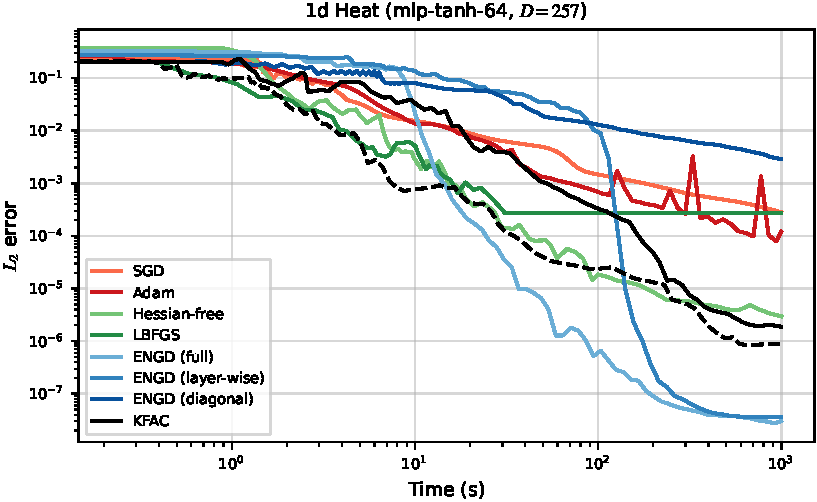
\includegraphics[trim={0 1.3cm 0 0},clip]{\pathToFigs/l2_error_over_time.pdf}
    % trim the legend and titles
    % [trim={left bottom right top},clip]
    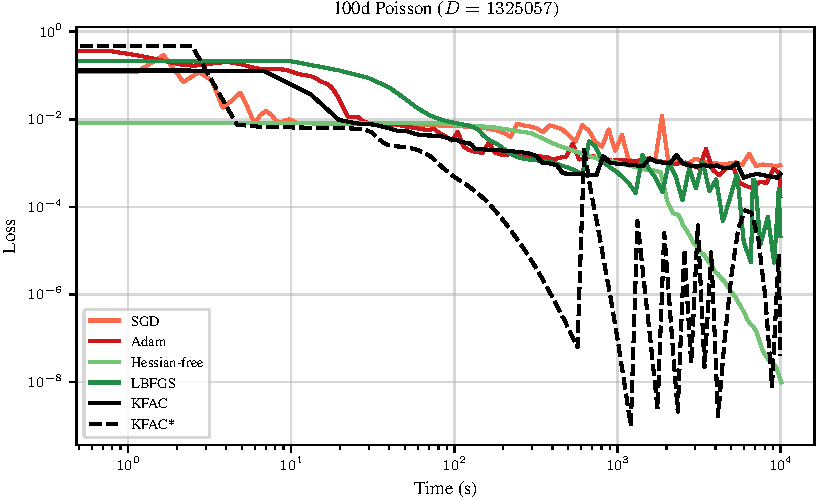
\includegraphics[trim={0 0.5cm 0 0.3cm},clip]{\pathToFigs/loss_over_time.pdf}
  \end{subfigure}
  \begin{subfigure}[t]{1.0\linewidth}
    \caption{}\label{subfig:fokker-planck-random-step}
    % trim the legend, xlabel and xticklabels
    % [trim={left bottom right top},clip]
    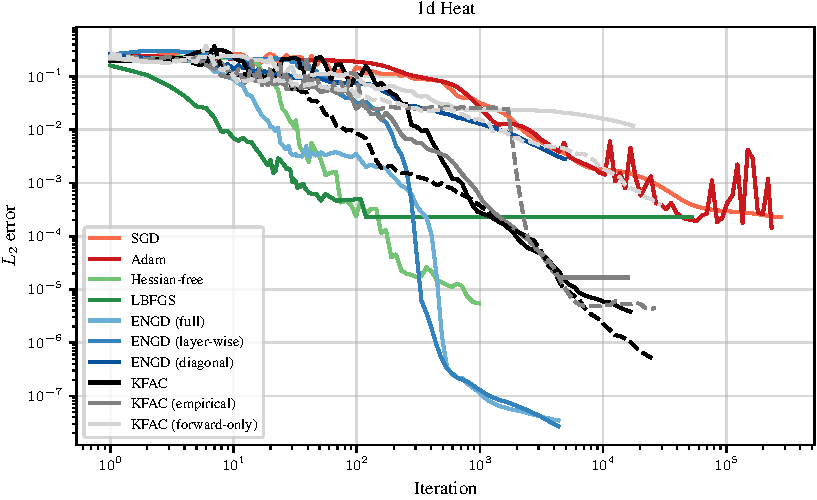
\includegraphics[trim={0 1.3cm 0 0.3cm},clip]{\pathToFigs/l2_error_over_step.pdf}
    % trim the titles
    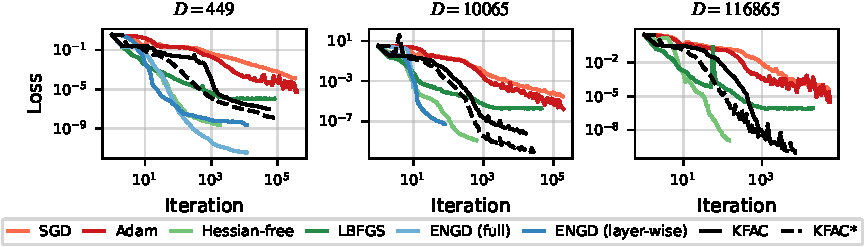
\includegraphics[trim={0 0 0 0.3cm},clip]{\pathToFigs/loss_over_step.pdf}
  \end{subfigure}
  \caption{Training loss and evaluation $L_2$ error for learning the solution to Fokker Planck (left) and logarithmic Fokker-Planck equations (center, right) over (\subref{subfig:fokker-planck-random-time}) time and (\subref{subfig:fokker-planck-random-step}) steps using random search.}\label{fig:fokker-planck-random-appendix}
\end{figure}

\paragraph{Best run details} The runs shown in \Cref{fig:fokker-planck-random-appendix} correspond to the following hyper-parameters:
\begin{itemize}
\item $1+1$-d Fokker-Planck equation with $2 \to 64 \to 1$ tanh-activated MLP ($D=\num{257}$):
  \begin{itemize}
    \def\pathToRuns{kfac_pinns_exp/exp46_fokker_planck1d_isotropic_gaussian_random/tex}
  \item \textbf{SGD:} learning rate: $\num[scientific-notation=true]{1.007555e-03}$, momentum: $\num[scientific-notation=true]{0.9}$
  \item \textbf{Adam:} learning rate: $\num[scientific-notation=true]{1.369294e-06}$, $N_{\Omega}$: $\num[scientific-notation=false]{203}$, $N_{\partial\Omega}$: $\num[scientific-notation=false]{1494}$, batch sampling frequency: $\num[scientific-notation=false]{9712}$
  \item \textbf{Hessian-free:} curvature matrix: $\text{GGN}$, initial damping: $\num[scientific-notation=true]{1.146081e-02}$, constant damping: $\text{no}$, maximum CG iterations: $\num[scientific-notation=false]{484}$, $N_{\Omega}$: $\num[scientific-notation=false]{2410}$, $N_{\partial\Omega}$: $\num[scientific-notation=false]{2448}$, batch sampling frequency: $\num[scientific-notation=false]{1311}$
  \item \textbf{LBFGS:} learning rate: $\num[scientific-notation=true]{0.2}$, history size: $\num[scientific-notation=false]{225}$
  \item \textbf{ENGD (full):} damping: $\num[scientific-notation=true]{1e-10}$, exponential moving average: $\num[scientific-notation=true]{0.3}$, initialize Gramian to identity: $\text{yes}$
  \item \textbf{ENGD (layer-wise):} damping: $\num[scientific-notation=true]{1e-06}$, exponential moving average: $\num[scientific-notation=true]{0.3}$, initialize Gramian to identity: $\text{no}$
  \item \textbf{KFAC:} damping: $\num[scientific-notation=true]{8.435180e-14}$, momentum: $\num[scientific-notation=true]{9.718645e-01}$, exponential moving average: $\num[scientific-notation=true]{9.800744e-01}$, initialize Kronecker factors to identity: $\text{yes}$, $N_{\Omega}$: $\num[scientific-notation=false]{2525}$, $N_{\partial\Omega}$: $\num[scientific-notation=false]{2663}$, batch sampling frequency: $\num[scientific-notation=false]{7916}$
  \item \textbf{KFAC*:} damping: $\num[scientific-notation=true]{2.965060e-08}$, exponential moving average: $\num[scientific-notation=true]{9.574717e-01}$, initialize Kronecker factors to identity: $\text{yes}$
  \end{itemize}

\item $9+1$-d logarithmic Fokker-Planck equation with $10 \to 256 \to 256 \to 128 \to 128 \to 1$ tanh-activated MLP ($D=\num{118145}$):
  \begin{itemize}
    \def\pathToRuns{kfac_pinns_exp/exp43_log_fokker_planck9d_isotropic_gaussian_random/tex}
  \item \textbf{SGD:} learning rate: $\num[scientific-notation=true]{1.007555e-03}$, momentum: $\num[scientific-notation=true]{0.9}$
  \item \textbf{Adam:} learning rate: $\num[scientific-notation=true]{1.369294e-06}$, $N_{\Omega}$: $\num[scientific-notation=false]{203}$, $N_{\partial\Omega}$: $\num[scientific-notation=false]{1494}$, batch sampling frequency: $\num[scientific-notation=false]{9712}$
  \item \textbf{Hessian-free:} curvature matrix: $\text{GGN}$, initial damping: $\num[scientific-notation=true]{1.146081e-02}$, constant damping: $\text{no}$, maximum CG iterations: $\num[scientific-notation=false]{484}$, $N_{\Omega}$: $\num[scientific-notation=false]{2410}$, $N_{\partial\Omega}$: $\num[scientific-notation=false]{2448}$, batch sampling frequency: $\num[scientific-notation=false]{1311}$
  \item \textbf{LBFGS:} learning rate: $\num[scientific-notation=true]{0.2}$, history size: $\num[scientific-notation=false]{225}$
  \item \textbf{KFAC:} damping: $\num[scientific-notation=true]{8.435180e-14}$, momentum: $\num[scientific-notation=true]{9.718645e-01}$, exponential moving average: $\num[scientific-notation=true]{9.800744e-01}$, initialize Kronecker factors to identity: $\text{yes}$, $N_{\Omega}$: $\num[scientific-notation=false]{2525}$, $N_{\partial\Omega}$: $\num[scientific-notation=false]{2663}$, batch sampling frequency: $\num[scientific-notation=false]{7916}$
  \item \textbf{KFAC*:} damping: $\num[scientific-notation=true]{2.965060e-08}$, exponential moving average: $\num[scientific-notation=true]{9.574717e-01}$, initialize Kronecker factors to identity: $\text{yes}$
  \end{itemize}
  We noticed that KFAC* requires exponential moving averages close to one to work well.
  We see that while KFAC reduces the loss roughly as well as KFAC* per iteration (\Cref{subfig:fokker-planck-random-step} center), its internal line search has detrimental effects on generalization (\Cref{subfig:fokker-planck-random-step} center) and run time (\Cref{subfig:fokker-planck-random-time} center).

\item $99+1$-d logarithmic Fokker-Planck equation with $10 \to 768 \to 768 \to 512 \to 512 \to 1$ tanh-activated MLP ($D=\num{1325057}$):
  \begin{itemize}
    \def\pathToRuns{kfac_pinns_exp/exp45_log_fokker_planck99d_isotropic_gaussian_random/tex}
  \item \textbf{SGD:} learning rate: $\num[scientific-notation=true]{1.007555e-03}$, momentum: $\num[scientific-notation=true]{0.9}$
  \item \textbf{Adam:} learning rate: $\num[scientific-notation=true]{1.369294e-06}$, $N_{\Omega}$: $\num[scientific-notation=false]{203}$, $N_{\partial\Omega}$: $\num[scientific-notation=false]{1494}$, batch sampling frequency: $\num[scientific-notation=false]{9712}$
    % \item \textbf{Hessian-free:} curvature matrix: $\text{GGN}$, initial damping: $\num[scientific-notation=true]{1.146081e-02}$, constant damping: $\text{no}$, maximum CG iterations: $\num[scientific-notation=false]{484}$, $N_{\Omega}$: $\num[scientific-notation=false]{2410}$, $N_{\partial\Omega}$: $\num[scientific-notation=false]{2448}$, batch sampling frequency: $\num[scientific-notation=false]{1311}$
  \item \textbf{LBFGS:} learning rate: $\num[scientific-notation=true]{0.2}$, history size: $\num[scientific-notation=false]{225}$
  \item \textbf{KFAC:} damping: $\num[scientific-notation=true]{8.435180e-14}$, momentum: $\num[scientific-notation=true]{9.718645e-01}$, exponential moving average: $\num[scientific-notation=true]{9.800744e-01}$, initialize Kronecker factors to identity: $\text{yes}$, $N_{\Omega}$: $\num[scientific-notation=false]{2525}$, $N_{\partial\Omega}$: $\num[scientific-notation=false]{2663}$, batch sampling frequency: $\num[scientific-notation=false]{7916}$
    % \item \textbf{KFAC*:} damping: $\num[scientific-notation=true]{2.965060e-08}$, exponential moving average: $\num[scientific-notation=true]{9.574717e-01}$, initialize Kronecker factors to identity: $\text{yes}$
  \end{itemize}
\end{itemize}

\paragraph{Search space details} The runs shown in \Cref{fig:fokker-planck-random-appendix} were determined to be the best via a random search on the following search spaces which each optimizer given approximately the same total computational time ($\mathcal{U}$ denotes a uniform, and $\mathcal{LU}$ a log-uniform distribution):
\begin{itemize}

\item $1+1$-d Fokker-Planck equation with $2 \to 64 \to 1$ tanh-activated MLP ($D=\num{257}$):
  \begin{itemize}
    \def\pathToRuns{kfac_pinns_exp/exp46_fokker_planck1d_isotropic_gaussian_random/tex}
  \item \textbf{SGD:} learning rate: $\mathcal{LU}([\num[scientific-notation=true]{1e-06}; \num[scientific-notation=false]{1}])$, momentum: $\mathcal{U}([\num[scientific-notation=false]{0}; \num[scientific-notation=true]{0.99}])$, $N_{\Omega}$: $\mathcal{C}(\{\num[scientific-notation=false]{100},\num[scientific-notation=false]{101},\text{\dots},\num[scientific-notation=false]{5000}\})$, $N_{\partial\Omega}$: $\mathcal{C}(\{\num[scientific-notation=false]{50},\num[scientific-notation=false]{51},\text{\dots},\num[scientific-notation=false]{2500}\})$, batch sampling frequency: $\mathcal{C}(\{\num[scientific-notation=false]{0},\num[scientific-notation=false]{1},\text{\dots},\num[scientific-notation=false]{1000}\})$
  \item \textbf{Adam:} learning rate: $\mathcal{LU}([\num[scientific-notation=true]{0.0001}; \num[scientific-notation=true]{0.5}])$
  \item \textbf{Hessian-free:} curvature matrix: $\mathcal{U}(\{\text{GGN},\text{Hessian}\})$, initial damping: $\mathcal{LU}([\num[scientific-notation=true]{1e-15}; \num[scientific-notation=false]{1}])$, constant damping: $\mathcal{U}(\{\text{no},\text{yes}\})$, maximum CG iterations: $\mathcal{U}(\{\num[scientific-notation=false]{1},\num[scientific-notation=false]{2},\text{\dots},\num[scientific-notation=false]{500}\})$, $N_{\Omega}$: $\mathcal{U}(\{\num[scientific-notation=false]{100},\num[scientific-notation=false]{101},\text{\dots},\num[scientific-notation=false]{5000}\})$, $N_{\partial\Omega}$: $\mathcal{U}(\{\num[scientific-notation=false]{50},\num[scientific-notation=false]{51},\text{\dots},\num[scientific-notation=false]{2500}\})$, batch sampling frequency: $\mathcal{U}(\{\num[scientific-notation=false]{0},\num[scientific-notation=false]{1},\text{\dots},\num[scientific-notation=false]{5000}\})$
  \item \textbf{LBFGS:} learning rate: $\mathcal{C}(\{\num[scientific-notation=true]{0.5},\num[scientific-notation=true]{0.2},\num[scientific-notation=true]{0.1},\num[scientific-notation=true]{0.05},\num[scientific-notation=true]{0.02},\num[scientific-notation=true]{0.01}\})$, history size: $\mathcal{C}(\{\num[scientific-notation=false]{75},\num[scientific-notation=false]{100},\num[scientific-notation=false]{125},\num[scientific-notation=false]{150},\num[scientific-notation=false]{175},\num[scientific-notation=false]{200},\num[scientific-notation=false]{225},\num[scientific-notation=false]{250}\})$
  \item \textbf{ENGD (full):} damping: $\mathcal{C}(\{\num[scientific-notation=true]{1e-08},\num[scientific-notation=true]{1e-09},\num[scientific-notation=true]{1e-10},\num[scientific-notation=true]{1e-11},\num[scientific-notation=true]{1e-12},\num[scientific-notation=false]{0}\})$, exponential moving average: $\mathcal{C}(\{\num[scientific-notation=false]{0},\num[scientific-notation=true]{0.3},\num[scientific-notation=true]{0.6},\num[scientific-notation=true]{0.9}\})$, initialize Gramian to identity: $\mathcal{C}(\{\text{no},\text{yes}\})$
  \item \textbf{ENGD (layer-wise):} damping: $\mathcal{U}(\{\num[scientific-notation=true]{0.01},\num[scientific-notation=true]{0.001},\num[scientific-notation=true]{0.0001},\num[scientific-notation=true]{1e-05},\num[scientific-notation=true]{1e-06}\})$, exponential moving average: $\mathcal{U}(\{\num[scientific-notation=false]{0},\num[scientific-notation=true]{0.3},\num[scientific-notation=true]{0.6},\num[scientific-notation=true]{0.9},\num[scientific-notation=true]{0.99}\})$, initialize Gramian to identity: $\mathcal{U}(\{\text{no},\text{yes}\})$
  \item \textbf{KFAC:} damping: $\mathcal{LU}([\num[scientific-notation=true]{1e-15}; \num[scientific-notation=true]{0.01}])$, momentum: $\mathcal{U}([\num[scientific-notation=false]{0}; \num[scientific-notation=true]{0.99}])$, exponential moving average: $\mathcal{U}([\num[scientific-notation=false]{0}; \num[scientific-notation=true]{0.99}])$, initialize Kronecker factors to identity: $\mathcal{C}(\{\text{no},\text{yes}\})$
  \item \textbf{KFAC*:} damping: $\mathcal{LU}([\num[scientific-notation=true]{1e-15}; \num[scientific-notation=true]{0.01}])$, exponential moving average: $\mathcal{U}([\num[scientific-notation=false]{0}; \num[scientific-notation=true]{0.99}])$, initialize Kronecker factors to identity: $\mathcal{U}(\{\text{no},\text{yes}\})$, $N_{\Omega}$: $\mathcal{U}(\{\num[scientific-notation=false]{100},\num[scientific-notation=false]{101},\text{\dots},\num[scientific-notation=false]{5000}\})$, $N_{\partial\Omega}$: $\mathcal{U}(\{\num[scientific-notation=false]{50},\num[scientific-notation=false]{51},\text{\dots},\num[scientific-notation=false]{2500}\})$, batch sampling frequency: $\mathcal{U}(\{\num[scientific-notation=false]{0},\num[scientific-notation=false]{1},\text{\dots},\num[scientific-notation=false]{5000}\})$
  \end{itemize}
\item $9+1$-d logarithmic Fokker-Planck equation with $10 \to 256 \to 256 \to 128 \to 128 \to 1$ tanh-activated MLP ($D=\num{118145}$):
  \begin{itemize}
    \def\pathToRuns{kfac_pinns_exp/exp43_log_fokker_planck9d_isotropic_gaussian_random/tex}
  \item \textbf{SGD:} learning rate: $\mathcal{LU}([\num[scientific-notation=true]{1e-06}; \num[scientific-notation=false]{1}])$, momentum: $\mathcal{U}([\num[scientific-notation=false]{0}; \num[scientific-notation=true]{0.99}])$, $N_{\Omega}$: $\mathcal{C}(\{\num[scientific-notation=false]{100},\num[scientific-notation=false]{101},\text{\dots},\num[scientific-notation=false]{5000}\})$, $N_{\partial\Omega}$: $\mathcal{C}(\{\num[scientific-notation=false]{50},\num[scientific-notation=false]{51},\text{\dots},\num[scientific-notation=false]{2500}\})$, batch sampling frequency: $\mathcal{C}(\{\num[scientific-notation=false]{0},\num[scientific-notation=false]{1},\text{\dots},\num[scientific-notation=false]{1000}\})$
  \item \textbf{Adam:} learning rate: $\mathcal{LU}([\num[scientific-notation=true]{0.0001}; \num[scientific-notation=true]{0.5}])$
  \item \textbf{Hessian-free:} curvature matrix: $\mathcal{U}(\{\text{GGN},\text{Hessian}\})$, initial damping: $\mathcal{LU}([\num[scientific-notation=true]{1e-15}; \num[scientific-notation=false]{1}])$, constant damping: $\mathcal{U}(\{\text{no},\text{yes}\})$, maximum CG iterations: $\mathcal{U}(\{\num[scientific-notation=false]{1},\num[scientific-notation=false]{2},\text{\dots},\num[scientific-notation=false]{500}\})$, $N_{\Omega}$: $\mathcal{U}(\{\num[scientific-notation=false]{100},\num[scientific-notation=false]{101},\text{\dots},\num[scientific-notation=false]{5000}\})$, $N_{\partial\Omega}$: $\mathcal{U}(\{\num[scientific-notation=false]{50},\num[scientific-notation=false]{51},\text{\dots},\num[scientific-notation=false]{2500}\})$, batch sampling frequency: $\mathcal{U}(\{\num[scientific-notation=false]{0},\num[scientific-notation=false]{1},\text{\dots},\num[scientific-notation=false]{5000}\})$
  \item \textbf{LBFGS:} learning rate: $\mathcal{C}(\{\num[scientific-notation=true]{0.5},\num[scientific-notation=true]{0.2},\num[scientific-notation=true]{0.1},\num[scientific-notation=true]{0.05},\num[scientific-notation=true]{0.02},\num[scientific-notation=true]{0.01}\})$, history size: $\mathcal{C}(\{\num[scientific-notation=false]{75},\num[scientific-notation=false]{100},\num[scientific-notation=false]{125},\num[scientific-notation=false]{150},\num[scientific-notation=false]{175},\num[scientific-notation=false]{200},\num[scientific-notation=false]{225},\num[scientific-notation=false]{250}\})$
  \item \textbf{KFAC:} damping: $\mathcal{LU}([\num[scientific-notation=true]{1e-15}; \num[scientific-notation=true]{0.01}])$, momentum: $\mathcal{U}([\num[scientific-notation=false]{0}; \num[scientific-notation=true]{0.99}])$, exponential moving average: $\mathcal{U}([\num[scientific-notation=false]{0}; \num[scientific-notation=true]{0.99}])$, initialize Kronecker factors to identity: $\mathcal{C}(\{\text{no},\text{yes}\})$
  \item \textbf{KFAC*:} damping: $\mathcal{LU}([\num[scientific-notation=true]{1e-15}; \num[scientific-notation=true]{0.01}])$, exponential moving average: $\mathcal{U}([\num[scientific-notation=false]{0}; \num[scientific-notation=true]{0.99}])$, initialize Kronecker factors to identity: $\mathcal{U}(\{\text{no},\text{yes}\})$, $N_{\Omega}$: $\mathcal{U}(\{\num[scientific-notation=false]{100},\num[scientific-notation=false]{101},\text{\dots},\num[scientific-notation=false]{5000}\})$, $N_{\partial\Omega}$: $\mathcal{U}(\{\num[scientific-notation=false]{50},\num[scientific-notation=false]{51},\text{\dots},\num[scientific-notation=false]{2500}\})$, batch sampling frequency: $\mathcal{U}(\{\num[scientific-notation=false]{0},\num[scientific-notation=false]{1},\text{\dots},\num[scientific-notation=false]{5000}\})$
  \end{itemize}

\item $99+1$-d logarithmic Fokker-Planck equation with $10 \to 768 \to 768 \to 512 \to 512 \to 1$ tanh-activated MLP ($D=\num{1325057}$):
  \begin{itemize}
    \def\pathToRuns{kfac_pinns_exp/exp45_log_fokker_planck99d_isotropic_gaussian_random/tex}
  \item \textbf{SGD:} learning rate: $\mathcal{LU}([\num[scientific-notation=true]{1e-06}; \num[scientific-notation=false]{1}])$, momentum: $\mathcal{U}([\num[scientific-notation=false]{0}; \num[scientific-notation=true]{0.99}])$, $N_{\Omega}$: $\mathcal{C}(\{\num[scientific-notation=false]{100},\num[scientific-notation=false]{101},\text{\dots},\num[scientific-notation=false]{5000}\})$, $N_{\partial\Omega}$: $\mathcal{C}(\{\num[scientific-notation=false]{50},\num[scientific-notation=false]{51},\text{\dots},\num[scientific-notation=false]{2500}\})$, batch sampling frequency: $\mathcal{C}(\{\num[scientific-notation=false]{0},\num[scientific-notation=false]{1},\text{\dots},\num[scientific-notation=false]{1000}\})$
  \item \textbf{Adam:} learning rate: $\mathcal{LU}([\num[scientific-notation=true]{0.0001}; \num[scientific-notation=true]{0.5}])$
    % \item \textbf{Hessian-free:} curvature matrix: $\mathcal{U}(\{\text{GGN},\text{Hessian}\})$, initial damping: $\mathcal{LU}([\num[scientific-notation=true]{1e-15}; \num[scientific-notation=false]{1}])$, constant damping: $\mathcal{U}(\{\text{no},\text{yes}\})$, maximum CG iterations: $\mathcal{U}(\{\num[scientific-notation=false]{1},\num[scientific-notation=false]{2},\text{\dots},\num[scientific-notation=false]{500}\})$, $N_{\Omega}$: $\mathcal{U}(\{\num[scientific-notation=false]{100},\num[scientific-notation=false]{101},\text{\dots},\num[scientific-notation=false]{5000}\})$, $N_{\partial\Omega}$: $\mathcal{U}(\{\num[scientific-notation=false]{50},\num[scientific-notation=false]{51},\text{\dots},\num[scientific-notation=false]{2500}\})$, batch sampling frequency: $\mathcal{U}(\{\num[scientific-notation=false]{0},\num[scientific-notation=false]{1},\text{\dots},\num[scientific-notation=false]{5000}\})$
  \item \textbf{LBFGS:} learning rate: $\mathcal{C}(\{\num[scientific-notation=true]{0.5},\num[scientific-notation=true]{0.2},\num[scientific-notation=true]{0.1},\num[scientific-notation=true]{0.05},\num[scientific-notation=true]{0.02},\num[scientific-notation=true]{0.01}\})$, history size: $\mathcal{C}(\{\num[scientific-notation=false]{75},\num[scientific-notation=false]{100},\num[scientific-notation=false]{125},\num[scientific-notation=false]{150},\num[scientific-notation=false]{175},\num[scientific-notation=false]{200},\num[scientific-notation=false]{225},\num[scientific-notation=false]{250}\})$
  \item \textbf{KFAC:} damping: $\mathcal{LU}([\num[scientific-notation=true]{1e-15}; \num[scientific-notation=true]{0.01}])$, momentum: $\mathcal{U}([\num[scientific-notation=false]{0}; \num[scientific-notation=true]{0.99}])$, exponential moving average: $\mathcal{U}([\num[scientific-notation=false]{0}; \num[scientific-notation=true]{0.99}])$, initialize Kronecker factors to identity: $\mathcal{C}(\{\text{no},\text{yes}\})$
    % \item \textbf{KFAC*:} damping: $\mathcal{LU}([\num[scientific-notation=true]{1e-15}; \num[scientific-notation=true]{0.01}])$, exponential moving average: $\mathcal{U}([\num[scientific-notation=false]{0}; \num[scientific-notation=true]{0.99}])$, initialize Kronecker factors to identity: $\mathcal{U}(\{\text{no},\text{yes}\})$, $N_{\Omega}$: $\mathcal{U}(\{\num[scientific-notation=false]{100},\num[scientific-notation=false]{101},\text{\dots},\num[scientific-notation=false]{5000}\})$, $N_{\partial\Omega}$: $\mathcal{U}(\{\num[scientific-notation=false]{50},\num[scientific-notation=false]{51},\text{\dots},\num[scientific-notation=false]{2500}\})$, batch sampling frequency: $\mathcal{U}(\{\num[scientific-notation=false]{0},\num[scientific-notation=false]{1},\text{\dots},\num[scientific-notation=false]{5000}\})$
  \end{itemize}
\end{itemize}

\subsection{Limitations of Our Current Approach}

\paragraph{Exact Initial Conditions*}
We can (and probably should) use a trick to automatically satisfy the initial conditions. To achieve this, we replace the neural network ansatz by
\begin{equation}
  (t,\vx)
  \mapsto
  t p_\vtheta(t,\vx) + p_0(\vx).
\end{equation}
By abuse of notation we again denote this function by $p_\vtheta$. This trick can also be used for the heat equation, of course. It is known in the literature and often facilitates training. \todo{This is currently difficult for our implementation, because we assume that the ansatz is a single neural network, not a sum. Is the $t$ above intended?}

\paragraph{Exact Initial Conditions*}
We can enforce initial conditions in the ansatz via
\begin{equation*}
  (t,\vx) \mapsto t q_\vtheta(t, \vx) + \log p_0(\vx)
\end{equation*}


%%% Local Variables:
%%% mode: latex
%%% TeX-master: "../main"
%%% End:
